\section{Program Control}

\subsection{Control Flow}

Programs for graphical user interfaces typically utilize some concept of
control flow between the user interface and the actual program logic,
often some kind of model view controller pattern.

However, when programs grow above a certain size the big picture usually
looks like a plate full of spaghetti containing some classes as
decoration.

\begin{figure}[ht]
\centering
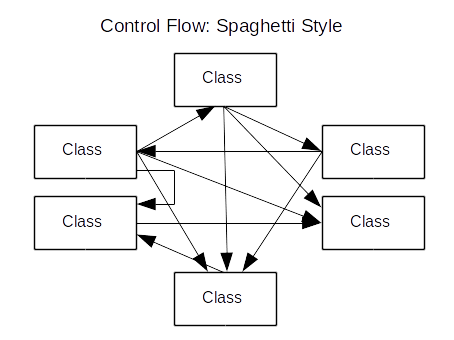
\includegraphics[width=12cm]{img/controlflowspaghetti.png}
\caption{Control Flow in a common program. Even well designed
programs have a tendency to end up looking like a plate full of spaghetti. }
\end{figure}

To help the programmer writing maintainable applications ui2go uses the
metaphor of a circular control flow. In this style of programming user
input is first directed to the graphical user interface (for example
clicking a button) and than forwarded to the program logic. The program
logic evaluates user input and updates the user interface, which is
observed by the user.

ui2go supports this style of coding by implementing a predefined flow of
events. The next section will go further into detail.

\begin{figure}[ht]
\centering
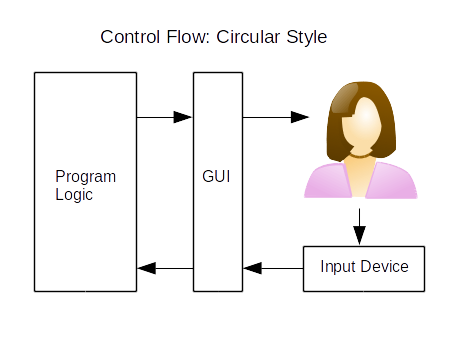
\includegraphics[width=12cm]{img/controlflowcircular.png}
\caption{ui2go supports a circular control flow, where user input
is transferred to the user interface and than to the program logic.
The program logic updates the user interface, which is observed by
the user.}
\end{figure}


\subsection{Events}

\subsubsection{General Idea}

In this world all complex organisms and societies have a hierarchical
structure. Larger systems are composed of smaller units (usually serving
a specific purpose) that are arranged in a hierarchical order. This
seems very natural to us and so we created technical systems according
to the same design. Here the units are often called modules.

The fact that hierarchical design is the result of millions of years of
evolution leads us to the conclusion that this design is somewhat
trustworthy. It is probably the best structure to reduce management
complexity in larger systems.

It is no surprise that computer programs were modelled in a hierarchical
way too. In the golden age of procedural programming a command was
resembled by a procedure that called other procedures further down the
hierarchy. This was called the top down approach in software
development. The top down approach worked very well for a while, but
programs had a tendency to grow in complexity and then graphical user
interfaces entered the scene.

One particular annoying problem with GUI programs is the non linear
control flow. The old style of programming worked very well for programs
that had a well defined entry point and processed data in a linear way
but in GUI programs user input can happen anytime anywhere and interrupt
the linear program execution.

This gave rise to a new style of programming: object orientation and the
massive use of events. This style is even closer to reality than top
down procedural programming. In reality anything can happen at anytime
(and it often does).

In real world hierarchical structures (biological organism, society,
organisation, military,...) commands and events have distinctive
meanings:

\begin{enumerate}
\item
  A command is given by someone who knows what to do. It travels
  downwards the hierarchy. Characteristics:

  \begin{itemize}
  \item
    Receiver (object)
  \item
    What to do (method name)
  \item
    Additional information (method parameters)
  \end{itemize}

  In object oriented programming a command is well resembled by a
  method.
\item
  An event is signalled by someone who does not know what to do. It
  travels upwards the hierarchy until it reaches some control instance
  who knows. An event often has multiple receivers. Characteristics:

  \begin{itemize}
  \item
    Sender (object raising the event)
  \item
    What has happened (kind of event)
  \item
    Additional information (event parameters)
  \item
    Time of the event. (This is only important is some cases, for
    example in distributed or multitasking environments where the
    original order of events might get lost)
  \end{itemize}

  In object oriented programming events are often modelled by function
  calls, which gives a totally wrong idea from a semantically point of
  view.
\end{enumerate}

\begin{figure}[ht]
\centering
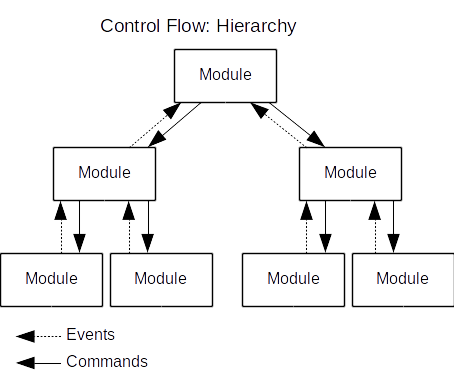
\includegraphics[width=12cm]{img/controlflowhierarchy.png}
\caption{Control flow in a hierarchical system. Events usually move
upwards the hierarchy and commands move downwards. If you don't like
the term module you can easily substitute it with department,
military unit or even class. }
\end{figure}

Imagine a town in medieval times. There were watchtowers at frequent
intervals to scan for enemies. The biggest enemy during these times was
probably fire. Fires broke out frequently and often destroyed large
parts of the town. The outbreak of a fire is a perfect example for an
event.

When the fire was spotted by a watchman (event dispatcher), he usually
shouted out loud \emph{Fire!} (event propagation) to warn the people and
to contact the fire department. At the fire department there was someone
who know what to do and he ordered some people to put out the fire.

Now lets turn to a more modern time example. An aircraft enters an
airspace. This event is monitored by several observers, a civilian air
traffic controller and a military air traffic control operator.

The civilian observer might feel a strong desire to guide the incoming
aircraft to safety, but if the pilot does not respond, he will assign
control to some military facility.

On the other hand the military air traffic control operator might have
observed the incident without the knowledge of the civilian controller
and already has taken actions. Intercepting planes are on their way. In
this case the message (event) from the civilian operator has no effect.

This example demonstrates that an event is no command and that it may be
fatal to handle an event like a command. In many programming
environments events are modelled as function calls and this suggests to
start the control flow at the source of the event.

But building a chain of command starting from the incoming aircraft is
like putting an enemy aircraft in control and that's clearly a bad idea.

I find it noteworthy that many textbooks about object oriented
programming totally neglect the notion of a proper hierarchy or modules.
They just deal with data structures (objects) and some design patterns
that are suited for programming in the small often leaving the
impression that objects happily communicate together on the same level.

But as programs grow larger, this approach no longer works and leads to
a mess of object calls that are hard to follow. I guess this is one of
the reasons why object oriented programs often gain a reputation of
being hard to maintain.

\subsubsection{Traditional Event Handling}

When events were introduced for graphical user interfaces event handling
was rather complicated. I showed some old style event handling code to a
bunch of people and they all agreed it looked surprisingly similar to
something like this:

\begin{verbatim}
ddkl?k$jj@d{alda
aldue)%%$kd§%hjg
df$!/kzhr)%§%@/}
\end{verbatim}

Some even insisted that the above code actually is traditional event
handling code.

It is easy to understand that nobody wanted to write code like this and
programmers hated to write programs with a graphical user interface.
They were in desperate need for a better solution and willing to take a
bet on everything that was different from the old style. In this
situation callback functions entered the scene (or at least the massive
use of callbacks).

\subsubsection{\label{callbackdesaster}Callback Disaster}

Because event handling was rather painful some smart people looked for a
more convenient solution and came up with something like this (pseudo
code):

\begin{verbatim}
// Handle click event from button
function onClick(event){
    // Do something useful with event
}

// Connect click event to function
button.onClick = onClick(event)
\end{verbatim}

This looks easy, doesn't it? Every other programmer thought the same and
event handling by using callback functions quickly became the standard
pattern in GUI programming.

Unfortunately what looks good in the small often is not as good in the
large and as programs got bigger some people started to realize that
there are a lot of problems associated with callback functions:

\begin{enumerate}
\item
  GUI and program code get mixed.

  This makes it hard to separate the concerns of user interface design
  and programming. It is also very hard to try out another interface
  design, because design and program are hardwired together.

  A maintainer who tries to grasp the program's control flow has to scan
  tons of user interface code, which has nothing to to with the actual
  program logic.
\item
  Strong coupling between components.

  This is not only the case for the user interface and the rest of the
  program. There are usually many callback functions weaving many
  connections between different components of the program. Thus it is
  hard to maintain or to implement changes in a certain module.
\item
  Control flow is hard to follow.

  The introduction of many callback methods makes the program's control
  flow hard to follow. Events often belong logically together, but
  callback methods rip this apart, creating a huge semantic gap between
  human understanding and the code.

  Some of these problems are usually being tackled by using some kind of
  model view controller pattern, but bigger programs still look like a
  big mess.
\item
  Inverted control flow.

  When it comes to big programs the program maintainer often has nothing
  to do with user interface design. This makes his job especially hard,
  because he has to take care of classes with no well defined entry
  points. So there is no concept of a control flow, that is easy to
  understand and could be followed.
\item
  Interdependencies between callback methods.

  Callback methods often introduce interdependencies, that make it
  necessary to introduce additional class variables. This makes the code
  hard to understand and hard to maintain.
\end{enumerate}

\begin{figure}[ht]
\centering
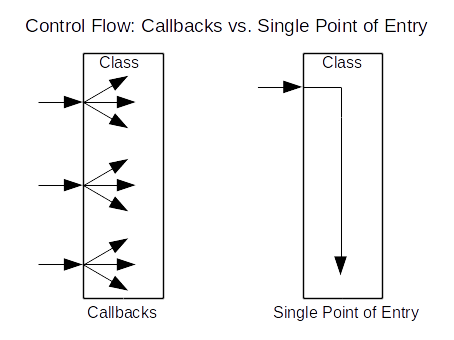
\includegraphics[width=12cm]{img/callbacks.png}
\caption{Control flow in a single class. The callback style is
confusing and hard to maintain. A single point of entry enables
a more traditional and easier linear control flow.}
\end{figure}

Now some people are looking for better solutions and try to get rid of
callback methods by whatever means possible, sometimes even introducing
new keywords to programming languages.

\subsubsection{ui2go Solution}

ui2go tries to solve the problems of callback functions by actually
taking one step back (Remember the big boots approach?). It fits
somewhere in between traditional event handling and callback methods,
but in a more modern form. The key features of ui2go event handling are:

\begin{enumerate}
\item
  A well defined flow of events.
\item
  Entry points into classes for groups of events.
\item
  Use of channels to handle associated events in a linear style.
\item
  I wish, I could write \emph{well structured events} here, but at the
  moment ui2go events are just a showcase.
\end{enumerate}

\begin{figure}[ht]
\centering
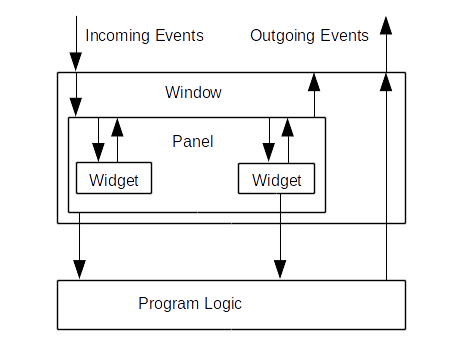
\includegraphics[width=12cm]{img/eventflow.png}
\caption{Event Flow in a ui2go program. The events flow from
the window down to the child widgets and after processing
again back up to the main window. At any given point the
program logic may be hooked into the event flow.}
\end{figure}

\pagebreak

\subsubsection*{Example: Window Event Handling using a Single Method}

This example presents a simple program for painting onto a canvas. It
shows, how mouse events are handled by a single method.

\begin{figure}[ht!]
\centering
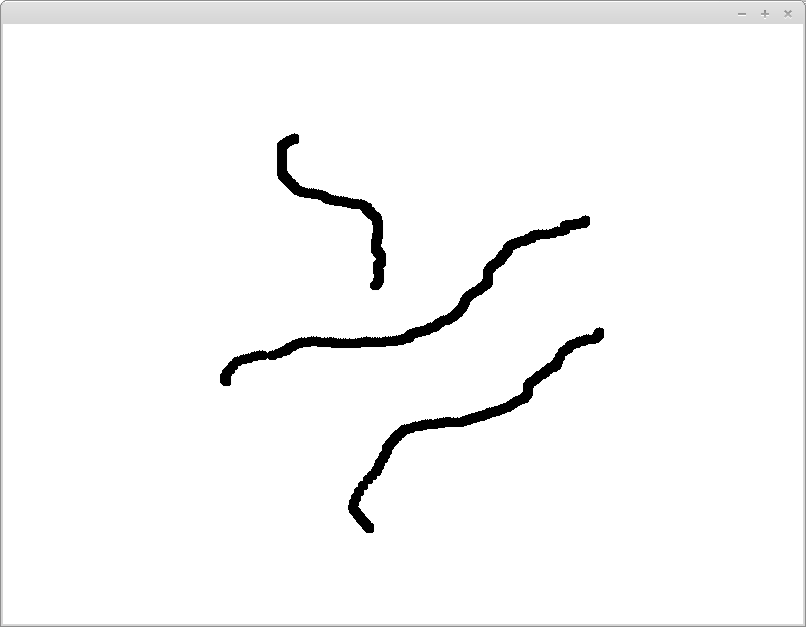
\includegraphics[width=12cm]{img/simplepaint.png}
\caption{An extremely simple program for painting.}
\end{figure}

Here is the complete source code:

\begin{verbatim}
// Package 02-paint implements a simple example on how to use
// the mouse for painting on a canvas.
package main

import (
    "code.google.com/p/ui2go/event"
    "code.google.com/p/ui2go/widget"
    "image"
)

// onEvent handles all events, that are sent from components
// embedded into the main window.
func onEvent(canvas *widget.Canvas, evt interface{}) {
    switch evt := evt.(type) {
    case event.PointerEvt:
        switch evt.Type {
        case event.PointerTouchEvt:
            canvas.MoveTo(image.Point{X: evt.X, Y: evt.Y})
        case event.PointerMoveEvt:
            if evt.State == event.PointerStateTouch {
                canvas.LineTo(image.Point{X: evt.X, Y: evt.Y})
            }
        }
    }
}

func main() {
    win := widget.NewWindow()
    canvas := widget.NewCanvas()
    // Layout one component in the window.
    win.Addf("%c growxy", canvas)
    // Redirect all events from the main window
    // to the onEvent method.
    event.NewReceiverFor(win).SetEvtHandler(
        func(evt interface{}) { onEvent(canvas, evt) })
    win.Show()
    win.Run()
}
\end{verbatim}

The line

\begin{verbatim}
    event.NewReceiverFor(win).SetEvtHandler(
        func(evt interface{}){ onEvent(canvas, evt) })
\end{verbatim}

creates a new event receiver for all window events and sets the
\texttt{OnEvent} method as it's event handler. The event handler is a
function, that processes the received events.

This coding style works fairly well, when there are only a few events to
manage, but when programs get bigger, it is more sensible to bundle
associated events together and to put them into a channel.

When events belong together, it is often useful to push them into a
channel. Retrieving events from a channel enables a linear coding style
and eliminates the need for class variables to keep track of event
interdependencies.


\subsubsection*{Example: Event Handling using a Channel}

This is a more advanced painting program as an example:

\begin{figure}[ht]
\centering
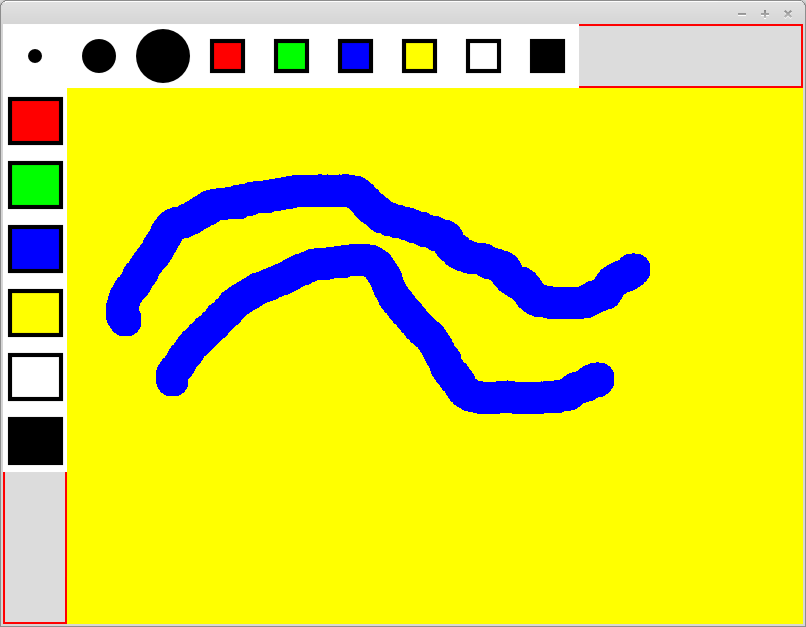
\includegraphics[width=12cm]{img/paint.png}
\caption{The paint program uses a channel to handle mouse
events from the canvas.}
\end{figure}

An excerpt from the source code:

\begin{verbatim}
// Connect events from canvas to onMouseEventsFromCanvas method.
event.NewReceiverFor(canvas).SetEvtChanHandler(
    func(ec <-chan interface{}){
        onMouseEventsFromCanvas(ec, canvas) })

func onMouseEventsFromCanvas(
    ec <-chan interface{}, canvas *widget.Canvas){
    for evt := range ec {
        switch evt := evt.(type) {
        case event.PointerEvt:
            switch evt.Type {
            case event.PointerTouchEvt:
                canvas.MoveTo(image.Point{X: evt.X, Y: evt.Y})
            case event.PointerMoveEvt:
                if evt.State == event.PointerStateTouch {
                    canvas.LineTo(image.Point{X: evt.X, Y: evt.Y})
                }
            }
        }
    }
}
\end{verbatim}

Connecting events to a function is nearly the same as in the previous
example, but this time the event handling function has a channel
argument:

\begin{verbatim}
    event.NewReceiverFor(canvas).SetEvtChanHandler(
        func(ec <-chan interface{}){
            onMouseEventsFromCanvas(ec, canvas)})
\end{verbatim}

This coding style has two major advantages: First, it is easy to process
events in linear style by using the \texttt{range} operator. There is no
need to react to external function calls, which makes the code very
legible.

Second, there is no need for extensive bookkeeping by using class
variables. Status information may be tracked by local variables, keeping
the code much clearer. The \texttt{isDrawing} variable is such a case.


\subsubsection*{Example: Old School Event Switching}

Some people will wonder, how events are distinguished inside an event
handler function. ui2go actually uses the old style of event switching:

\begin{verbatim}
    event.NewReceiverFor(buttonPanel).SetEvtHandler(
        func(evt interface{}){ onCommand(evt) })

    func onCommand(evt interface{}) {
        switch evt.Command {
        case "SmallBrush":
            canvas.SetBrushRadius(7)
        case "BigBrush":
            canvas.SetBrushRadius(27)
        }
    }
\end{verbatim}

Many programmers don't like this style. They find it ugly and inelegant.
I agree to that view, when it comes to long \texttt{if else} statements,
but I think Go \texttt{switch} statements are very legible.

But wouldn't it be much better to directly connect events to call back
functions? Most GUI libraries use this new style of coding (again in
pseudo code):

\begin{verbatim}
    smallBrushButton.onClick = onSmallBrushClick(evt)
    bigBrushButton.onClick = onBigBrushClick(evt)

    function onSmallBrushClick(evt){
        canvas.SetBrushRadius(7) 
    }

    function onBigBrushClick(evt){
        canvas.SetBrushRadius(27) 
    }
\end{verbatim}

Despite it's widespread use, this style has a number of drawbacks:

\begin{enumerate}
\item
  The problems associated with callback functions that were already
  discussed in section \ref{callbackdesaster}.
\item
  Did I already mention, that interface design and program code often
  get mixed up?
\item
  Method inflation: Code often consists of an extensive amount of one
  liners, making it harder to maintain. This problem could be overcome
  by binding events directly to closures, but this is usually considered
  bad style, because methods must often be called from different
  locations in the program code.
\item
  Program semantics are torn apart. Logically associated things are no
  longer associated in the source code.
\end{enumerate}

The old school code on the other side features some advantages:

\begin{enumerate}
\item
  Easy to read and maintain.
\item
  Easy to add scripting capabilities (just connect more event senders to
  the same event switch). The event switch already is some kind of
  simple interpreter.
\item
  Flexible code: For example, adding a new event handler just requires
  an extra case in the \texttt{switch} statement. It keeps the changes
  local to one class. The new style requires a new event connection and
  a new method. In bigger program this is usually done in different
  classes.
\item
  Network transparency could be achieved just by exchanging the event
  senders and listeners implementation.
\end{enumerate}

